%----------------------------------------
\begin{frame}
  \frametitle{What this talk is about} \small

To check anything, you need {\bf two artifacts}:

\vspace{0.35cm}

{\centering
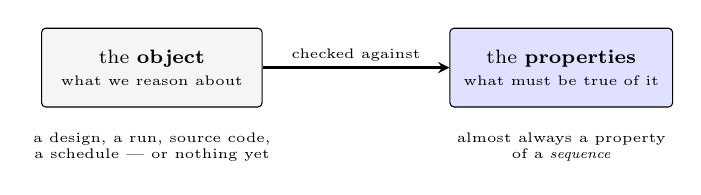
\begin{tikzpicture}[
  font=\scriptsize, >=stealth,
  b/.style={draw, rounded corners=1.5pt, align=center, inner sep=5pt,
            minimum height=1.0cm, minimum width=2.8cm},
  lab/.style={font=\tiny, align=center, inner sep=2pt}
]
  \node[b, fill=black!4]  (obj)  at (0,0)    {the {\bf object}\\{\tiny what we reason about}};
  \node[b, fill=blue!12]  (prop) at (5.2,0)  {the {\bf properties}\\{\tiny what must be true of it}};

  \node[lab, anchor=north] at (0,-0.75)   {a design, a run, source code,\\a schedule --- or nothing yet};
  \node[lab, anchor=north] at (5.2,-0.75) {almost always a property\\of a {\em sequence}};

  \draw[->, thick] (obj) -- node[font=\tiny, above, inner sep=2pt] {checked against} (prop);
\end{tikzpicture}\par}

\pause
\vspace{0.75cm}

Both must be written in a notation a machine can read.

\end{frame}

%----------------------------------------
\begin{frame}
  \frametitle{Five methods} \small

\vspace{-0.1cm}

\begin{center}\scriptsize
\renewcommand{\arraystretch}{1.25}
\setlength{\tabcolsep}{4pt}
\begin{tabular}{|>{\raggedright\arraybackslash}p{1.7cm}%
                |>{\raggedright\arraybackslash}p{2.1cm}%
                |>{\raggedright\arraybackslash}p{2.15cm}%
                |>{\raggedright\arraybackslash}p{2.4cm}|}
\hline
\rowcolor{blue!10}
{\bf Method} & {\bf Object} & {\bf Coverage} & {\bf Tools}\\
\hline
\rowcolor{orange!14}
\multicolumn{4}{|l|}{{\bf dynamic analysis} --- the system runs}\\
\hline
{\icontest[0.75]}\newline testing & the real system & one run per test & \ours{\fuzz{}}\\
\hline
{\iconrv[0.75]}\newline runtime verification & one real execution & that run, exactly & \ours{\tc{}, \daut{},
                                                                \pycontract{},
                                                                \dejavu{}}\\
\hline
\rowcolor{orange!14}
\multicolumn{4}{|l|}{{\bf static analysis} --- the system does not run}\\
\hline
{\iconcs[0.75]}\newline coding standards & source code & all runs, approximated & \comm{JPL checkers}\\
\hline
{\iconmc[0.75]}\newline model checking & a finite-state model & all runs of the {\em model} & \spin{},
                                                                     \tlaplus{},
                                                                     \ours{JPF1}\\
\hline
{\icontp[0.75]}\newline theorem proving & a mathematical model & all runs, unbounded & \lean{}, \zthree{},
                                                                     \esbmc{},
                                                                     \ours{\tasksat{}},
                                                                     \ours{\fcheck{}},
                                                                     \ours{\eva{}},
                                                                     \ours{K}\\
\hline
\end{tabular}
\end{center}

\vspace{-0.1cm}

\hfill {\scriptsize \ours{our tools} \quad \comm{commercial}}

\end{frame}
